\chapter{Design}\label{design}
\todo[inline]{Anna: skitser, navigation structure tree}
The aim of this chapter is to design the architecture components which will eventually guide the implementation of the system.

This chapter is divided into the following parts: Architecture Design, Application Method, and Component Design.
The Architecture Design in \cref{sec:architecturedesign} will introduce and discuss the criteria and the requirement priorities.
In the Application Method section, the main framework that the system will be implemented within is introduced and discussed.
This will be followed by the framework that has been chosen for the implementation of the system. % Henrik: Er dette ikke bare en gentagelse af linjen før? :-)
In Component Design in \cref{sec:componentdesign}, the theory for component design will be introduced, followed by the project's architecture component design.

\section{Architecture Design} \label{sec:architecturedesign}
In this section all of the pieces needed to be able to make the final component design are presented.
It starts with the system's criteria in \cref{sec:architecturecriteria}, followed by a prioritization of the system's requirements with the help of the MoSCoW rules in \cref{sec:requirements}.
After this, the system application framework is presented.

\documentclass[../../master.tex]{subfiles}
\begin{document}
\subsection{Criteria}\label{sec:architecturecriteria}
A good software system is one that meets its requirements and has no major weaknesses \citep[p.~179]{Rod-Aalborg}.
This system's requirements are listed and prioritized in \cref{sec:requirements} and the efforts put into avoiding weaknesses are laid out in this section.

Due to the conditions this system is developed under, see \cref{factor}, flaws are to be expected.
To minimize the amount of critical flaws the \textit{criteria} \citep[p.~180]{Rod-Aalborg} upon which the system will be judged have been prioritized.
The idea is that development will be focused on the 'very important' and 'Important' criterias to make sure that all of these work.
Less effort will be put into the 'Less important' and 'Irrelevant' criteria, making flaws in these areas more likely.
However, as established, they are less important and therefore the flaws will, most likely, not be critical.
Similarly, 'Easily fulfilled' will have less of a focus, but as the requirements are easily fulfilled critical flaws are not very likely.
These priorities can be found in \cref{fig:criteria} and the reasoning behind them follows below.

\begin{table}[H]
	\begin{center}
		\begin{tabular}{|l|c|c|c|c|c|}
			\hline
			Criteria $\backslash$ priority & \rotatebox{90}{Very important} &  \rotatebox{90}{Important} & \rotatebox{90}{Less important} & \rotatebox{90}{Irrelevant} & \rotatebox{90}{Easily fulfilled}\\
			\hline
			Usable & \xmark & & & & \\
			\hline
			Secure & & & & \xmark & \\
			\hline
			Efficient & & & & & \xmark \\
			\hline
			Correct & & \xmark & & & \\
			\hline
			Reliable & \xmark & & & & \\
			\hline
			Maintainable & & & \xmark & & \\
			\hline
			Testable & & \xmark & & & \\
			\hline
			Flexible & & & & \xmark & \\
			\hline
			Comprehensible & & \xmark & & & \\
			\hline
			Reusable & & & \xmark & & \\
			\hline
			Portable & & & & \xmark & \\
			\hline
			Interoperable & & & & \xmark & \\
			\hline
		\end{tabular}
	\end{center}
	\caption{Prioritized list}\label{fig:criteria}
\end{table}

It is very important that the system is \textbf{usable}.
As has been described in the previos chapters, \cref{sec:PACT-people}, the users may have limited IT experience, and the users in the reader role will get limited exposure to the system, only using it to read new editions of the handbook and marking it as read.

While the administrator or writer role will use the system more often, they too have limited IT experience, so the complexity should still be kept to a minimum in their case.

Ipsen has expressed that whether or not the system is \textbf{secure} is no major concern as the information is not confidential.
In the use case envisioned with the user, the program is only accessible inside a secured network, and it has therefore been determined that security is outside this systems area of responsibility and then irrelevant.

As the existing workflow is incredibly inefficient due to the amount of manual work it requires and no matter how inefficient the new system is it is very unlikely that it should be less \textbf{efficient}. Therefore this criterion is determined as easily fulfilled.

The \textbf{correct} criteria from \cref{fig:criteria} covers whether or not the system fulfills the system definition, that was specified in \cref{sec:systemdefinition}, and meets all the requirements, see \cref{sec:requirements}.
The reasoning for labeling 'correct' as important instead of very important is because of the long list of requirements where not all elements are equally important.

It is very important that the system is \textbf{reliable} as it is a problem if the system malfunctions and e.g. deletes files, assigns wrong version numbers or automatically approves a new version.
It could, should any of these happen, mean the company will lose their certification which, as described in \cref{sec:standards}, is at best a problem for consumers' trust to the company and at worst a requirement by law.

Whether the system is \textbf{maintainable} is less important as it is assumed that the user is not capable of maintaining it anyway.

The system needs to be \textbf{testable} in order to verify that it is reliable.
Therefore this is important.

According to the \textit{OOA\&D} method \citep[p.~182]{Rod-Aalborg}, it is very important that a system is \textbf{flexible}.
On the ohter hand, as the project will only be developed for half a year, this does not take priority and has been classifield as irrelevant.
The system is, however already developed with some future elements in mind: The changelog, which Ipsen has requested, is not a requirement under the current conditions, however it is a change which she assumes will happen within the next ten years or so, as stated in \cref{sec:CaseDescription}.

It is important that the code is \textbf{comprehensible} as we are seven diffferent people with varying areas of expertise and skill working on the same code simultaneously and we all need to understand it.

As stated before it seems unlikely that this project will be developed further after its completion and therefore the \textbf{reusability} is less of a concern.
However, the system is structured so that components can be reused to implement some of the requirements classified as 'Want to have but Won't have this time around', see \cref{sec:requirements} for the list.
This is most obvious with the abstract role class, which has remained even though it has no purpose in the current layout of the system.
As a result this criteria has been defined as less important.

As tablets and mobile phones are not allowed in the production, and it is assumed that the majority of employees use a standard internet browser, it is irrelevant whether or not the system is \textbf{portable}.

It is also irrelevant whether or not the system is \textbf{interoperable} as the only systems it needs to interoperate with are sms and e-mail, which it has been designed for from the start as an integral feature.

To summarize the top prioritized criteria are the systems usability and reliability.
Less important but still notable are correctness, testability and comprenhensibility.
These criteria will therefore be in focus when designing the components the system is made up of.
\end{document}

\subsection{MoSCoW rules}\label{sec:requirements}
It is important to prioritize a system's requirements after the first draft of a system has been designed.
This is because there are no guarantees that all of the requirements and design ideas are doable within the time frame of a given project.
The information in this chapter is based upon Benyon \cite{Benyon}.

These priorities are set to determine which requirements are absolutely necessary for the system to function, the \textit{minimal viable product} (MVP),
and which requirements are simply nice to include.
The \textit{MoSCoW rules}
have been chosen to help prioritize the requirements for this project.
The MoSCoW rules classifies these priorities into:

\begin{itemize}
    \item \textit{Must have}.
    \item \textit{Should have}.
    \item \textit{Could have}.
    \item \textit{Want to have but Won’t have this time around}.
\end{itemize}

Must haves are the fundamental requirements to include where system would not function without.
Must haves also determines the MVP.
Should haves are essential requirements to include if the time frame allowed, but the system could still function without.
Could haves are less important requirements than must haves and should haves and they would easily be excluded from the system.
Want to have but Won't haves are requirements that can wait until a later point of the system development.

For the sake of preventing misunderstandings the definition for requirement used in this report \citep[p.~147]{Benyon} can be found in \cref{defn:Req} below.

\begin{defn}\label{defn:Req}
    A requirement is something the product must do or a quality that the product must have
\end{defn}

\subsubsection{Defining requirements} \label{sec:requirementsdefinition}
It was in \cref{sec:PACT} mentioned how it is important, when designing an interactive system, to do it with the users in mind.
Therefore, before defining a project's requirements it is essential to figure out the client's wants and needs.
A lot of different techniques can be used when defining a project's requirements, e.g.:

\begin{itemize}
    \item Interviews
    \item Observing people and record their activities on video
    \item Organizing focus groups
\end{itemize}

These techniques can help designers to better understand the problems the client has with their current system, and at the same time, give a better understanding of the requirements for the new system.
Using these techniques where the designer interacts with other people also provides them with a lot of stories that can form the basis for the analysis work.
Even though a designer have all these techniques at their disposal, the interview technique
is one of the most effective techniques to find out what the client wants and needs.

The process of defining a project's requirements is an iterative process, see \cref{sec:iterativModel}.
This is because new requirements will pop-up throughout the design process.
This may happen when the user interacts with the system during tests and it becomes clear misunderstandings of the basic concept has happend.
Furthermore, it may also happen when the user realises other needs than what was thought necessary of the system to begin with.

For this project the interview technique was used to define this project's requirements, see \cref{sec:firstinterview}. This helped defining the prioritization of the following requirements:

\begin{itemize}
    \item
    Must have:
        \begin{itemize}
            \item
            The system must manage versions of handbook documents
            \item
            A \textit{Table of Contents} (TOC) with title, ID number, date and version number
            \item
            The system must be able to handle PDF files
            \item
            Title and ID number are linked
            \item
            Once a version has been added to the handbook, it cannot be changed
        \end{itemize}
    \item
    Should have:
        \begin{itemize}
			\item
			Automatic updates of TOC
            \item
            A human-written changelog may be depending on the company settings
            \item
            Registration of who among specific employees have read a version
            \item
            The handbook should be printable.
            \item
            Different levels of access rights to the documents within the handbook
            \item
            Readers and writers only have access to the newest version of a document
            \item
            Administrators have acces to all features supported by the system, except marking versions as read
            \item
            It should be possible to group users into departments, and associate them to documents.
            \item
            It should be simple to switch from an exsisting system, and back again
                \todo[inline]{RASMUS: Tjek om den her formulering passer med FACTOR, omformuler til kvantitativt krav}
        \end{itemize}
    \item
    Could have:
        \begin{itemize}
            \item
            When a document is updated, a notification could be sent out to the associated departments.
            \item
            The system could be able to handle documents of different file-types
            \item
            Option to sort documents according to different attributes
            \item
            System for approval of new versions of documents
			\item
			Be able to fill a PDF header with information such as approvers and valid date
        \end{itemize}
    \item
    Want to have but Won't have this time around:
        \begin{itemize}
            \item
            Highlight differences between current and previous versions.
            \item
            Approval of suppliers and their documents.
        \end{itemize}
\end{itemize}

The requirements belonging to this category are necessary since the system would not be functional without them.
The first item under \textit{must have} which is ''The system should manage versions of handbook documents'' is intentionally broad as it is expanded upon in the following four items.

The following prioritization \textit{Should have} contains very important requirements that the system must include if Ipsen were to use the solution.
The reason that these requirements are placed here is because the system is technically able to function as a management software without these specific requirements.

The last priorizations \textit{Could have} and \textit{Want to have but Won't have this time around} are the least important requirements in relation to the system.
These items are placed under these priorities as they would be nice to include in the system, but Ipsen does not consider them vital to the solution or her problem.


\section{Application Method}\label{sec:AppMethod}

\subsection{Web Applications}
% Ideen her er meget afgrænsning. Rummet af alle arkitekturer bliver afgrænset til noget der bruger netværk, til noget der bruger klient-server, til web
In this section the application method will be discussed and at the end a specific application method is chosen.

The requirements in the system definition state that users should be able to work together through the system, independent of geography.
%Anna: Hvor står det henne???, gerne sætte en reference ind)
%Anja: Det er nærmere en reference til PACT, der skal sættes in ovenfor
The OOA\&D method designates that in these scenarios, the client-server model should be considered.
% Røde aalborg, side 202
In this scenario, at least communication between clients is required.
%Anna: Evt i stedet for at bruge scenario to gange i streg brug "development project" eller bare "project".
Many of the features in the system definition, such as having multiple users being able to access the same handbook, registering whether the document has been read, and certainty of the version being read being recent, is impossible without some sort of communication between clients.
%Anna: synes det bliver en meget lang sætning, er det bare mig?
The possible forms of communication are, in broad terms, a decentralized approach and a centralized approach.
%Anna: er det ikke enten eller frem for både og?

It is, however, pretty clear that a centralized approach is ideal.
A decentralized system is more difficult to develope and manage.
%anna: Evt i stedet for difficult bruge complex? (ikke noget jeg har stærke følelser om)
Where democratic systems fit well with a decentralized system, this is far from this type application.
%Anna: hvorfor virker det ved democratic systems og ikke her?
%Anna: Hvorfor er det pretty clear centralized er bedre for det her system (Evt snakke om sikkehed ift firma hemmeligheder (kunne være et forslag))
Then what is left is to decide how the client and server applications look, and what the advantages or disadvantages are.
The two possibilities are roughly; a web application, or a desktop application that speaks to a server.
While a desktop application is often faster, and has bigger opportunities for interacting with the hardware, it is also harder to manage on the users computer and keep the application up to date on each machine.
Whereas, the application logic for a web-app will be constantly updated, as the part of the application that is currently used is downloaded to the users computer as a part of each request.
%Anna: Synes denne sætning på en elelr anden måde bliver mere kringlet end nødvendigt (er det bare mig)?
The web-app can be thought of as an additional layer of abstraction that does away with platform specific issues, such as adapting to different operating systems.
A disadvantage of web-apps is the requirement of there being a server, and the possible loss of the ability to work if it is down.
However, since the application already requires a server, this is a smaller problem.

The largest disadvantage, and quite possibly one that has not been considered enough in this development project, is the learning curve associated with web applications.
The web builds on a lot of technologies, CSS, Javascript and HTML, which are absolutely necessary, but can be difficult to learn all at once.

The model decided upon here is that of loccal presentration.
As the integrity of the data is incredibly important, all business logic should be centrally administrated, and that way be resilient to user error.
Choosing a local presentation model allows us to create a web application.
%Anna: igen for at fjerne 'we' kan der skrives "Choosing a local presentation model allows for the creation of a web application.
A web application has many advantages, including but not limited to, mature UI, easy cross platform support, and avoiding having to install anything.

A web application is any form of application where the client runs in a web browser.
%anna: hvilken client snakkes der om lige her?
This section will take a general overview of how web applications are structured, and what can be done to ensure stability.
%Anna: Er den sætning lige ovenfor ikke malplaceret det er vel det der lige er blevet gennemgået?
%Jeg tænker, at vi også skal skrive om hvilke andre platforme og metoder der kunne anvendes til at udforme systemet.

\documentclass[../../master.tex]{subfiles}
\begin{document}
\subsection{ASP.NET Core} \label{sec:aspnetcore}

ASP.NET core is a web framework developed by Microsoft for developing web applications in the .NET Core Framework \cite{aspnetcore2}.
ASP stands for \textit{Active Server Pages} and offers a variety of application models, one of which being the Model-View-Controller (MVC) pattern.
The framework has built-in support for many common features, such as database integration, identity and authorization with multi-factor, external authentication and CSS frameworks.

The reason for this web API to be used is because of it is part of the scope of the development project to develop an application using the programming language C\#.
ASP.NET Core supports, among others, C\# and is able to integrate the language with a web application.
It uses a MVC design pattern, \cref{sec:mvc}, as a basis for the architecture of the applications developed in it.

ASP.NET Core is a web framework developed by Microsoft, for developing web applications in the .NET Core framework.
%Anja: Er der en grund til, at det ovenstaaende staar der igen? :P
The framework is quite widely used, which means that there are plenty of modules available for doing many jobs. 
% Anja: Jeg bryder mig heller ikke om koblingen at "Fordi det bliver brugt meget -> saa er der mange moduler". Det er lidt en falsk logik
Besides that, the framework has built-in support for many common features, such as database integration, identity and authorization with multi-factor and external authentication, CSS frameworks, and much more.
% Anja: Gentagelse
It uses the quite popular MVC design pattern as a basis for the architecture of the applications developed in it.

\subsubsection{Model-View-Controller design pattern}\label{sec:mvc}
The MVC pattern is an architectural pattern that splits an application into three basic components; the model, the view, and the controller.
Originally meant for Graphical User Interface (GUI) development, the pattern has been adapted into web development, and is used by many of the frameworks in the space. \cite{gangoffour}

The advantages of using the MVC architecture are that it helps reducing the complexity of the application by dividing its components into three individual components each with its own function and responsibilites.
These components are as mentioned before \textit{model, view}, and \textit{controller}, see \cref{fig:MVC-components}.
Furthermore the MVC archictecture supports test driven development and also does not use server-based forms which gives the developers full control over the application. \cite{mvcarticle}

\begin{figure}[H]
\centering
	\begin{tikzpicture}[node distance=2cm]
	\node[process] (model) {Model};
	\node[process] (view) [below of=model, left of=model] {View};
	\node[process] (controller) [below of=model, right of=model] {Controller};
	\draw[arrow] (model.south west) -- node[left] {Updates} (view.north);
	\draw[arrow] (controller.north) -- node[right] {Updates} (model.south east);
	\node[process] (user) [below of=model, node distance=3.5cm] {User};
	\draw[arrow] (view.south) -- node[left] {Perceives} (user.north west);
	\draw[arrow] (user.north east) -- node[right=0.2cm] {Interacts with} (controller.south);
	\end{tikzpicture}
	\caption{The Model-View-Controller design pattern.}\label{fig:MVC-components}
\end{figure}

The model component's responsibility is to implement the logic of the data domains \cite{mvcarticle}.
In other words it is here the main algorithms reside that which provide the solutions for the main function of the application.
The responsibility of the view component is to provide an interface for the user and makes it possible for the user to interact with the application.
The controller component's responsibility is to respond to the user's request and gives a means to make the applications underlying algorithms and logics accessible for the user. \cite{mvcarticle}

The MVC architecture is thus a three-layered structure where each component is loosely dependent on each other.
This gives the developers a possibility of developing each component simultaneously.
This separation between the components also makes it easier to test the application in the test-driven development approach. \cite{mvcarticle}

The data managed by the application is encapsulated into the model classes.
These can then be accessed or subscribed to by the views, which the user sees.
The user then subsequently interacts with the controller, which in turn updates the model.
The seperation of concerns allows for a quite flexible architecture, where you can change the view without touching the model or controller, or the controller without changing the view and model.\cite{gangoffour}

\subsection{Entity Framework}\label{sec:efcore}

Entity Framework (EF) is a framework for mapping object-oriented data structures into a relational database, also referred to as an object-relational mapping framework, for .NET.{\color{red}\cite{efcore}}
The job of the EF is translating the objects in memory into Structured Query Language (SQL) statements so that these objects can be stored in a database.
\begin{figure}[H]
	\centering
	\begin{tikzpicture}[node distance=1cm, minimum height=0.6cm]
		\node[process] (net) {ASP.NET Core};
		\node[process] (efcore) [below=0.5cm of net] {Entity Framework Core};
		\node[process] (sql) [below=0.5cm of efcore] {Relational Database};
		\draw[arrow] (net) -- (efcore);
		\draw[arrow] (efcore) -- (net);
		\draw[arrow] (sql) -- (efcore);
		\draw[arrow] (efcore) -- (sql);
	\end{tikzpicture}
	\caption{The relationship between ASP.NET Core and the Relational Database, with the EF acting as a glue between the two layers}\label{fig:ASP-Entity}
\end{figure}

To use the EF, everything needed to do in the code is to provide a context object.
which mediates the connection, giving the configuration arguments a connection to a database requires.
This context defines the sets of objects to be stored in the database, and also the database to be used.
The EF supports multiple kinds of databases, from MariaDB to PostgreSQL.
The support for multiple database systems is provided by the respective database providers.
\end{document}

\documentclass[../../master.tex]{subfiles}
\begin{document}
\subsection{Database}
Jan Paredaens et al. \cite{RelationalDatabaseModel} defines a database system as a collection of programs that run on a computer and that help the user to get information, to update information, to protect information, in general to manage information.

Overall, there exist three different types of database \cite{RelationalDatabaseModel}:

\begin{itemize}
    \item
    \textit{Network model} where the structure of information is represented by a directed graph.
    \item
    \textit{Hierarchical model} where the information is represented as a set of trees.
    \item
    \textit{Relational model} where the information is represented in tables.
\end{itemize}

Relational databases are one of the most popular where, as mentioned above, the data is organized in tables with rows and columns.\cite{OracleWhatIsDatabase}
The application discussed in this report is using such a type of database due to it being the best supported in ASP.NET Core.

To get a better understanding of how the data is structured in a relational database imagine a system with a lot of users.
This system might be interested in keeping track of the users \textit{username, password, firstname, lastname} and \textit{email}.
In a relational database this information can be represented as follows:

\begin{table}[H]
    \centering
    \begin{tabular}{lllll}
        USERNAME & PASSWORD & FIRSTNAME & LASTNAME & EMAIL \\
        \hline
        username1 & pw123 & Billy & Johnson & bj@mail.com \\
        username2 & pw456 & Lucy & Johnson & lj@mail.com \\
    \end{tabular}
    \caption{Table of users}
\end{table}

Structuring the users like this makes it easy to add new users to the table since the number of columns does not change, nor their names.

The most common way to interact with a database is to use SQL.
SQL is a database sublanguage that differs from other computer languages because it describes what the computer \textit{should do} rather than \textit{how it should do it}.\cite{SQLIntroduction}

SQL makes it easy to perform Create, Read, Update, Delete (CRUD) operations on the database.\cite{OracleWhatIsDatabase}
An example of how to use SQL could be someone who wants to retrieve complete infromation about all the users from the user table

\begin{lstlisting}[caption={An SQL query that fetches complete information for every user}, label=lstSQL-user1]
SELECT * FROM USER;
\end{lstlisting}

Or maybe this person is just interested in retrieving a specific user

\begin{lstlisting}[caption={An SQL query that only fetches complete information for username1}, label=lstSQL-user2]
SELECT * FROM USERS WHERE username = "username1";
\end{lstlisting}

It has now been explained what a database is, how it works and how to interact with the database.
The next section will move from backend technologies, to explaining front-end technologies.

\end{document}


\section{Component Design} \label{sec:componentdesign}

In this section the component design theory will be introduced and elaborated.
This theory will be utilized in the following section where the component design for the system will be presented.
%Anna: evt fjerne sætningen ovenfor da det virker til at være en gentagelse af den første

\subsection{Components}


\subsection{System design} \label{sec:systemdesign}

In relation to the ASP.NET MVC pattern there are immediate similarities to the component design theory in \cref{archicomponents}.
There can among other be drawn parallels between the \textit{model} component and the \textit{model} classes in the MVC pattern.
The possible parallels are listed in the table below.

\begin{table}
	\centering
	\begin{tabular}{| c | c | }
	\hline
	\textbf{Components} & \textbf{MVC Pattern} \\
	\hline
	Model & Model \& EF Core \\
	\hline
	Functionality & Controller \\
	\hline
	Interface & View \\
	\hline
\end{tabular}
\caption{{\color{red}indsæt caption tekst}}\label{tab:PatternParallels}
\end{table}

As written in the component design theory in \cref{sec:archicomponents} the model components should seek to solve the problem of the problem domain.
%Anna: enten henvis til specifikke definition hvis sådan en eksisterer ellers henvis til afsnittet.
%Anna: Mener vi virkeligt "problem og the problem domain"
The model component in the MVC pattern is likewise going to contain the classes and objects that seeks to solve the problem domain through meeting the requirements written in {\color{red}section xx}.
The model component in the implementation is among other classes going to contain \textit{documents, users, departments, versions, approvals} and \textit{read statuses}.
The arguments for including these classes can be seen in \cref{sec:classdiagram}.
The database in form of EF Core is also included in the model component as this in part also seeks to solve the problem domain.
%Anna: Vi hrar endnu ikke introdyuceret denne forkortelse i brødteksten(EF core)

As written in the component design theory the responsibilty of the functionality is to provide the actor a means to access the model component.
%Anna: Henvis til afsnitet
%Anja: Der er blevet henvist i paragraffen ovenfor. Det begynder at blive overkill
The controller component in the MVC pattern does this by communicating between the model component and the view component.
The controllers retrieves data from the database and both methods and objects from the models.
Hereafter,it links these to the view.

The responsibility of the interface component is the handle the interaction between the users and the functionality.
This is done through the view model in the MVC pattern as the interface is handled in big part due to HTML, CSS and JavaScript.
These are what determines what the actors sees and what they can interact with.

\subsection{Component layers}
In relation to the theory written in \cref{archicomponents} the components can be designed in layers to describe their responsibilities and relation to each other.
The components in the MVC pattern with EF Core included can also be designed with the layered architecture in mind.
To give an overview and understanding of the architecture and design a simple component layer design can be seen in the figure below:
%Anna: synes den sidste sætning bliver en smule kringlet

\begin{figure}[H]
	\centering
	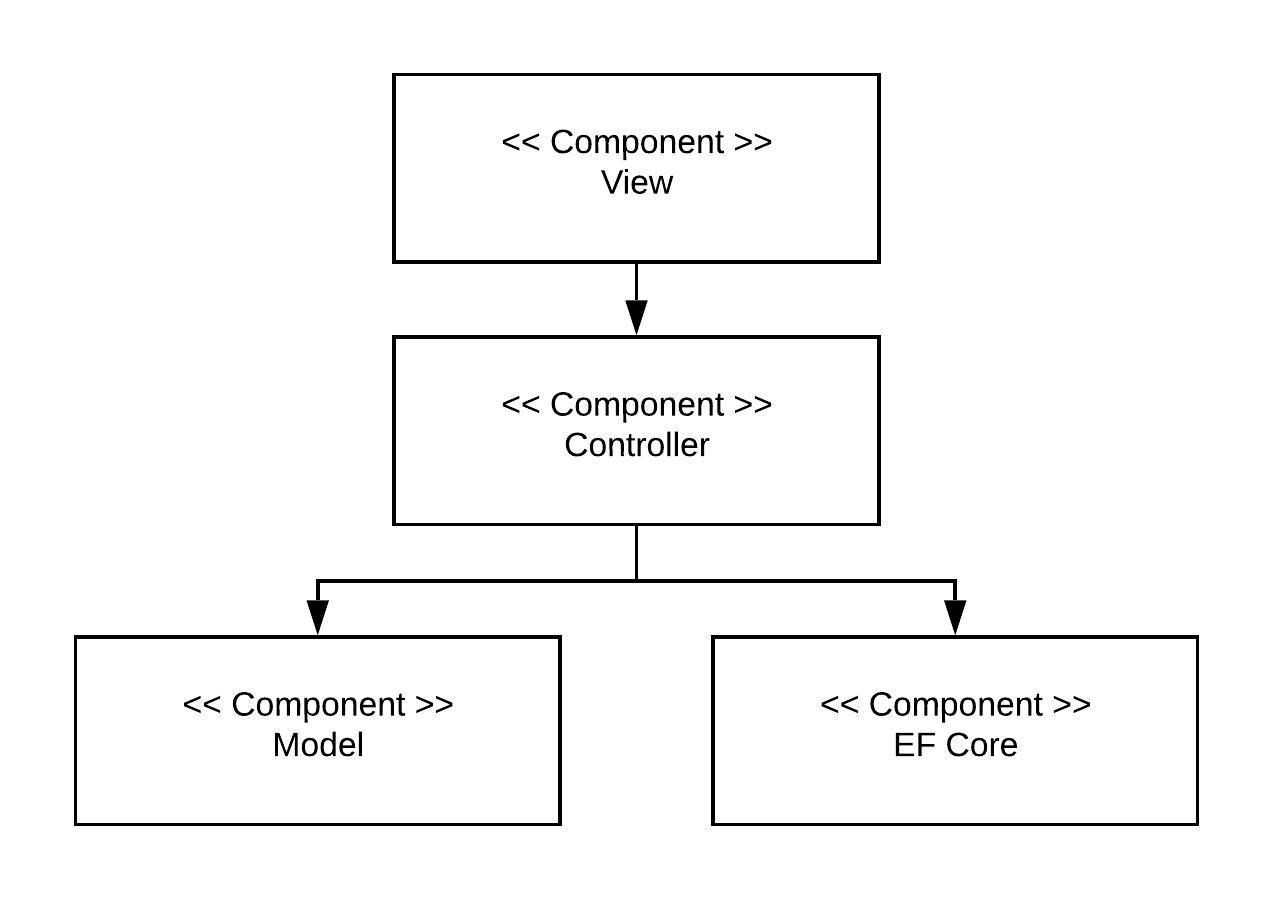
\includegraphics[width=0.7\textwidth]{billeder/simplecomponents.jpeg}
	\caption{Simple component layer design}\label{fig:SimpleComponent}
\end{figure}

View, controller, model, and EF Core are thus the main components layers that can be found in the design, each with a well-defined responsibility.
Ideally the architecture is designed so that the view and model components do not have to interact with each other.
% Kilde? Det virker lidt suspekt at views og models ikke skal kunne snakke med hinanden
% Anja: Virkelig? Tjah, saa tænker jeg slet sætningen ovenfor, da den er trukket ud af min røv
It is the intention that the controller is the link between these components, which is why it is placed in the middle of the layer components.
The main function of the controller is to link objects from the model component and data from the EF Core database and make these accessible for the view component.

%Anna: vil vove at påstå der ikke birde være et afsnit her
% Anja: Jeg vil paastaa det modsatte
This will not always be the case as the ASP.NET Core MVC model is designed so that a view has a corresponding controller.
For example the document view will have a corresponding document controller.
The document view will eventually have to borrow objects and data from other models in the system, which means that the view will at times have to bypass the controller component to communicate with the model component.

Subsystems can be explored from the main components, which e.g. are the interface system and its underlying technologies.
These are HTML, CSS, JavaScript and razor.
The model component has two main parts which are the model classes from the MVC pattern and the EF Core database system.
These two are defined as separate components which share similar responsibilities in the model component.
These components their relations with each other, and their underlying sub components can be seen in the complex version of the layer design below:

\begin{figure}[H]
	\centering
	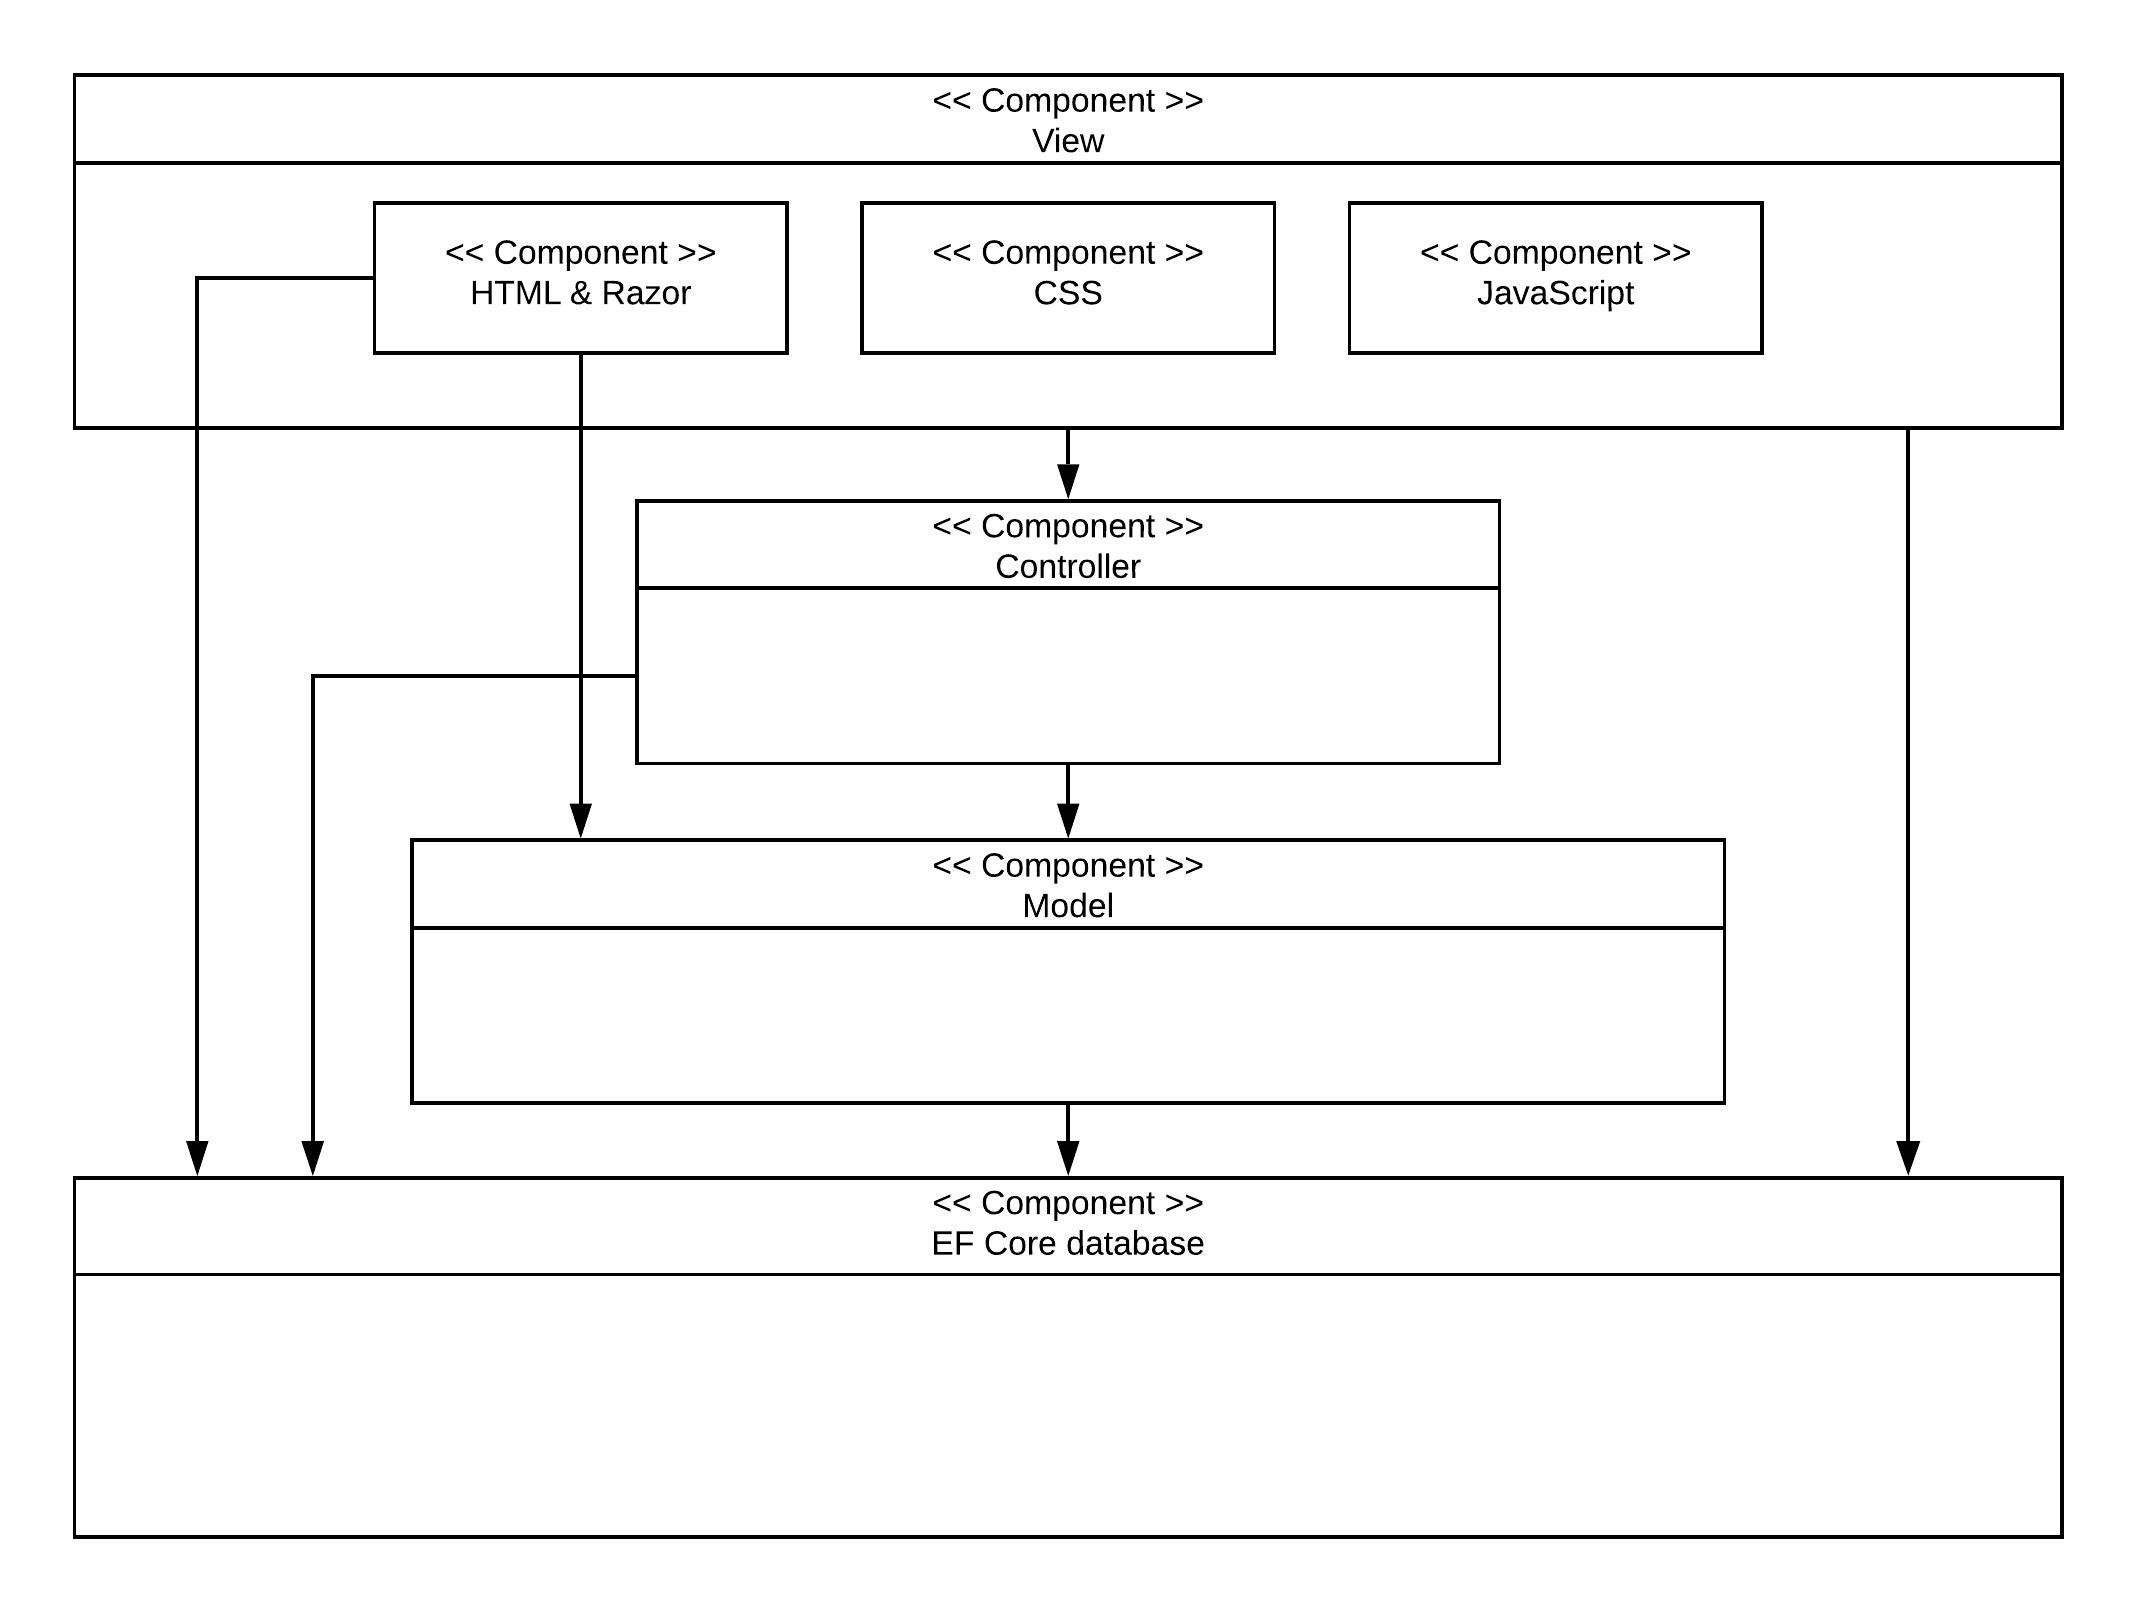
\includegraphics[width=1\textwidth]{billeder/complexcomponents.jpeg}
	\caption{Complex component layer design}
\end{figure}

Ideally the design would have \textit{closed-relaxed} architecture as the components would only be able to access layers adjacent to them.
In this design the design would be \textit{relaxed} as the controller would have access to both the view and the model components.
As it is though the design has an \textit{open-relaxed} architecture as the view component occasionally has access to the model component.
%Anna: Kan godt tænkes de to sidste sætninger trænger til en omskrivning
% Anja: Tjoh
% Henrik: Tænker at det er forkert med pil fra JavaScript til Model

In the final design there will be several classes included within each of the components.
Each of the main classes in the model component will have a corresponding controller and view in relation to it.
For example the document class in the model component will have a corresponding database in EF Core as well as a corresponding controller and view.
Here the documents object is within the model component and the documents data will be stored in the database.
A corresponding controller, which mainly handles the document class, ensures that the class and database are accessible for the actor.
The corresponding view ensures that the actor is able to see and interact with the document classes and database.

\section{Navigation Tree}
This section describes the navigation tree that visualizes how user move through the application, see \Cref{fig:Navigation}.
\begin{figure}
	\centering
	\begin{tikzpicture}[align=center, scale=1.0, transform shape]
		\node(login)[predefined]{Login};
		\node(activate)[predefined, right=0.4cm of login, yshift=0.7cm]{Activate\\account};
		\node(main)[predefined, right=0.4cm of activate, yshift=-0.7cm]{Main};
		
		\node(user-a)[predefined, right=0.4cm of main, yshift=-1.4cm]{User\\administration};
			\node(create)[predefined, right=0.4cm of user-a, yshift=0.7cm]{Create\\user};
			\node(user-i)[predefined, right=0.4cm of user-a, yshift=-0.7cm]{User\\info};
			\node(edit)[predefined, right=0.4cm of user-i]{Edit};
		\node(depart)[predefined, below=1.7cm of user-a]{Departments};
			\node(dep-detail)[predefined, right=0.4cm of depart]{Detail};
			\node(edit-U)[predefined, right=0.4cm of dep-detail, yshift=0.7cm]{Edit\\users};
			\node(edit-D)[predefined, right=0.4cm of dep-detail, yshift=-0.7cm]{Edit\\documents};
		\node(setting)[predefined, below=0.7cm of depart]{Settings};
		
		\node(archive)[predefined, right=0.6cm of main, yshift=1.0cm]{Archive};
			\node(preview)[predefined, right=0.6cm of archive]{Preview\\document};
		\node(approvals)[predefined, above=0.7cm of archive]{Approvals};
		\node(doc)[predefined, above=0.7cm of approvals]{Add new\\document};
		
		\node(fit)[draw=red, fit=(main) (edit-D) (doc) (setting)] {};
		\node(profile)[predefined, right=0.4cm of fit, yshift=0.7cm]{Edit\\profile};
		\node(out)[predefined, right=0.4cm of fit, yshift=-0.7cm]{Log\\out};
		
		\draw[black](login.east) -| (0.8,-0.7);
		\draw[black](0.8,-0.7) |- (activate.west);
		\draw[black](activate.east) -| (2.8,0.0);
		\draw[black](0.8,-0.7) -| (2.8,0.0);
		\draw[black](2.8,0.0) |- (main.west);
		\draw[black](main.east) -| (4.4,0.1);
		\draw[black](4.4,0.1) |- (doc.west);
		\draw[black](4.4,0.1) |- (approvals.west);
		\draw[black](4.4,0.1) |- (archive.west);
		\draw[black](main.east) -- (4.6,0.0);
		\draw[black](4.4,0.1) |- (user-a.west);
		\draw[black](4.4,0.1) |- (depart.west);
		\draw[black](4.4,0.1) |- (setting.west);
		\draw[black](6.7,0.5) |- (approvals.east);
		\draw[black](6.7,0.5) |- (archive.east);
		\draw[black](6.7,0.5) |- (4.6,0.0);
		\draw[black](6.7,0.5) |- (preview.west);
		\draw[black](7.6,-0.9) |- (user-a.east);
		\draw[black](7.6,-0.9) |- (user-i.west);
		\draw[black](7.6,-0.9) |- (create.west);
		\draw[black](user-i.east) |- (edit.west);
		\draw[black](depart.east) -- (dep-detail.west);
		\draw[black](dep-detail.east) -| (9.1,-3.5);
		\draw[black](edit-U.west) -| (9.1,-3.5);
		\draw[black](edit-D.west) -| (9.1,-3.5);
		\draw[black](fit.east)-| (11.7, 0.0);
		\draw[black](profile.west)-| (11.7, 0.0);
		\draw[black](out.west)-| (11.7, 0.0);
			
	\end{tikzpicture}
	\caption{Navigation tree}\label{fig:Navigation}
\end{figure}


The user will first encounter the Login page.
For the first-timer user they have to enter the Activate account page and insert the given username received from administrator to register email address (optional) and create a password.
Once activate account process is finished user will be redirected to the handbook's Main page.
If the account is already activated user will be redirected to the Main page once logged in.

In the Main page administrator and writer will be able to access the ``Add new document'' page.
Writer will be able to access awaiting approvals under the relevant document section in the Main page.
Administrator will be able to enter the Approvals page through a sidebar which is only accessible for administrator.
The sidebar consists of:

\begin{itemize}
	\item Handbook (return to the Main page)
	\item Approvals
	\item Archive
	\item User administration
	\item Departments
	\item Settings
\end{itemize}

The Preview document page can be access in three ways depends on access rights, see \Cref{tab:docPreviewEntries} below.

\begin{table}[H]
	\begin{center}
	\begin{tabular}{| m{20em} | c | c | c | c | c |}
		\hline
		Document preview entry & Administrator & Writer & Reader \\
		\hline
		 Directly through document in the valid handbook & x  & x & x\\
		\hline
		 Through archive document  & x &  & \\
		\hline
		 Via awaiting approval document & x & x &  \\
		\hline
	\end{tabular}
	\end{center}
	\caption{Document preview entries}\label{tab:docPreviewEntries}
\end{table}

Through the User administration page which is accessible from the sidebar administrator will be able to access the Create user page or the User info page to enter the Edit page and update user information.

Under the Departments page entered through the sidebar.
Administrator will be able to click on existing department name to enter the Detail page of an overview of associate users and documents.
In the Detail page administrator would be able to enter the Edit users page or the Edit documents page.

The Settings page is accessible from the sidebar where administrator can change the company name and enable or disabled changelog functionality to the application.

In the Navigation tree in \Cref{fig:Navigation} the red box indicate that every role can enter the Edit profile page or Log out on the global, top-level navigation bar anywhere in the navigation flow within the red box.

%GUI
